\documentclass[tikz,border=2pt]{standalone}
\usepackage{amsmath,amssymb}
\usepackage{tikz}

\begin{document}
% The event A is cut into the pieces A ∩ B_i by a partition; adding the pieces gives P(A),
% and each piece can be computed as P(A | B_i) P(B_i).
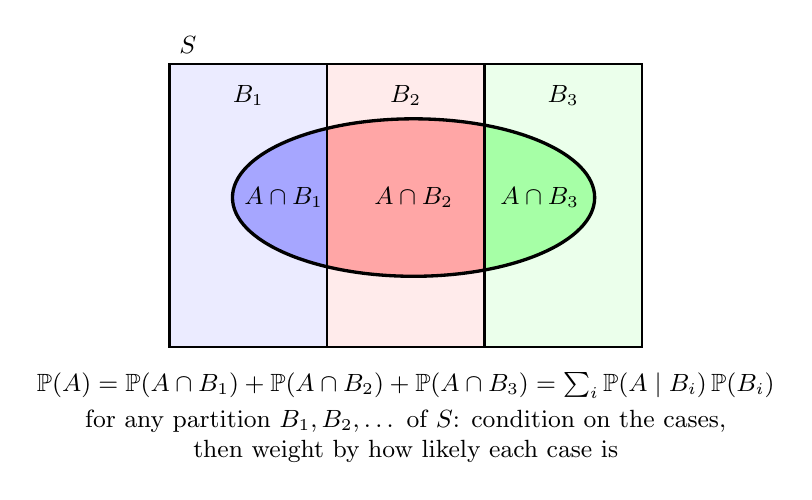
\begin{tikzpicture}[every node/.style={font=\small}]
	\fill[blue!8] (-3,-1.8) rectangle (-1,1.8);
	\fill[red!8] (-1,-1.8) rectangle (1,1.8);
	\fill[green!8] (1,-1.8) rectangle (3,1.8);
	\begin{scope}
		\clip (0.1,0.1) ellipse (2.3 and 1.0);
		\fill[blue!35] (-3,-1.8) rectangle (-1,1.8);
		\fill[red!35] (-1,-1.8) rectangle (1,1.8);
		\fill[green!35] (1,-1.8) rectangle (3,1.8);
	\end{scope}
	\draw[thick] (-3,-1.8) rectangle (3,1.8);
	\draw[thick] (-1,-1.8) -- (-1,1.8);
	\draw[thick] (1,-1.8) -- (1,1.8);
	\draw[very thick, black] (0.1,0.1) ellipse (2.3 and 1.0);
	\node at (-2,1.4) {$B_1$};
	\node at (0,1.4) {$B_2$};
	\node at (2,1.4) {$B_3$};
	\node at (-1.55,0.1) {$A\cap B_1$};
	\node at (0.1,0.1) {$A\cap B_2$};
	\node at (1.7,0.1) {$A\cap B_3$};
	\node[anchor=south west] at (-3,1.8) {$S$};
	\node[anchor=north, align=center] at (0,-2.0) {$\mathbb{P}(A)=\mathbb{P}(A\cap B_1)+\mathbb{P}(A\cap B_2)+\mathbb{P}(A\cap B_3)=\sum_i \mathbb{P}(A\mid B_i)\,\mathbb{P}(B_i)$\\[2pt] for any partition $B_1,B_2,\dots$ of $S$: condition on the cases,\\ then weight by how likely each case is};
\end{tikzpicture}
\end{document}
